\documentclass[utf8]{beamer}
\usepackage{listings}
\usepackage[russian]{babel}
\usetheme{Malmoe}
\title{Мультиплексирование}
\author {Компьютерные сети и протоколы}
\date{Лекция 4-5}
\begin{document}
%--------------------------------------------------------------------------------
\begin{frame}
\titlepage
\end{frame}
%--------------------------------------------------------------------------------
\begin{frame}
\begin{block}{NRZ -- Без возвращения к нулю (USB)}
\begin{center}
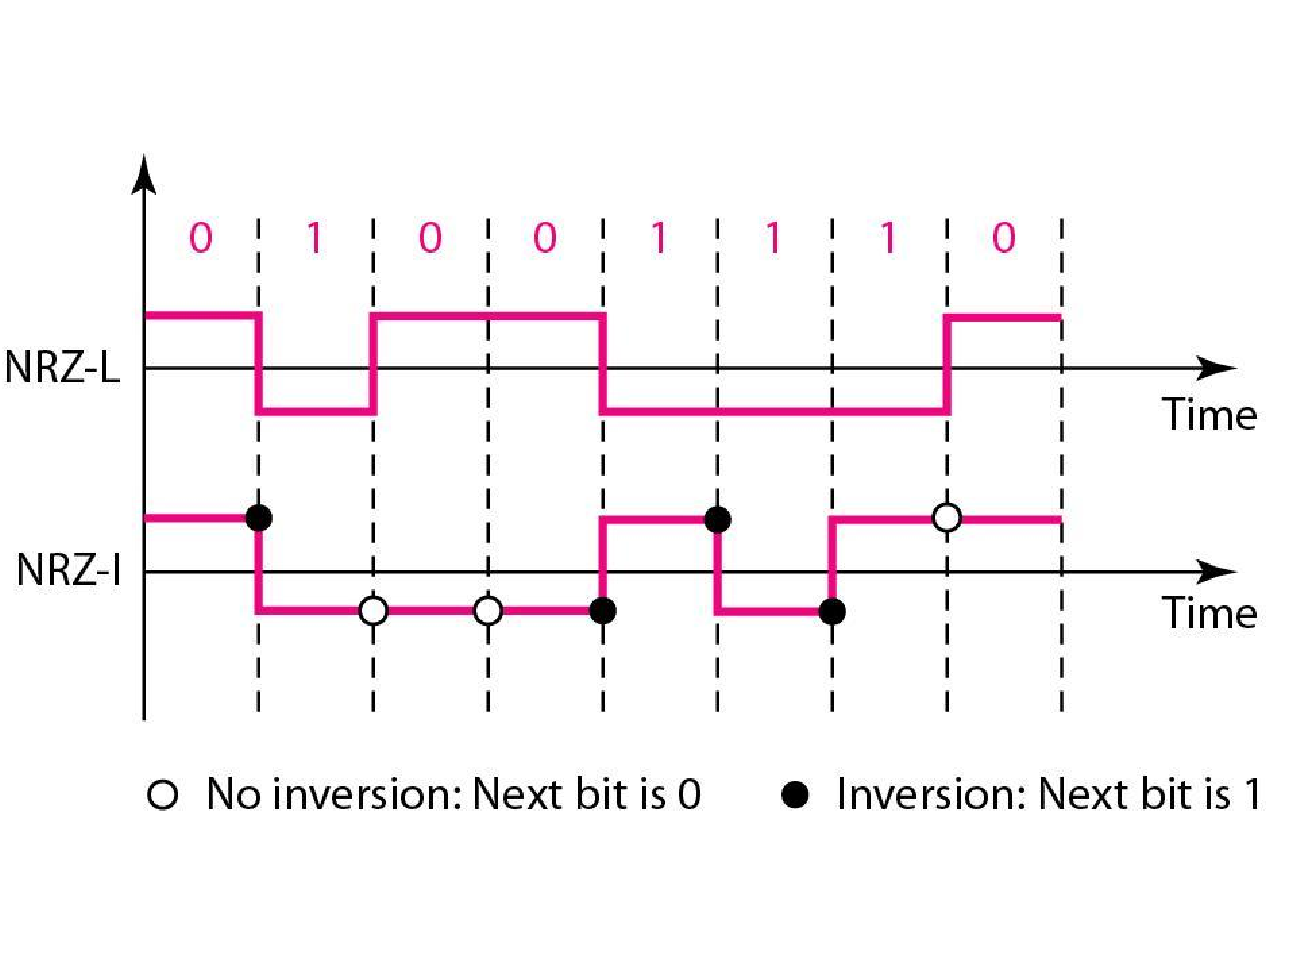
\includegraphics[width=0.5\textwidth]{pic/NRZ.png}
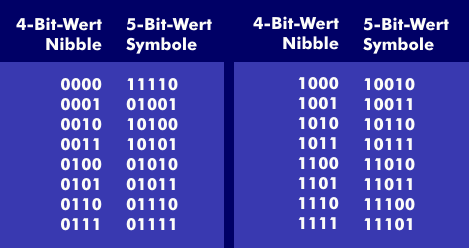
\includegraphics[width=0.3\textwidth]{pic/4b-5b.png}
\end{center}
\end{block}
\begin{block}{Манчестерский код: $Data \otimes Clock$}
\begin{center}
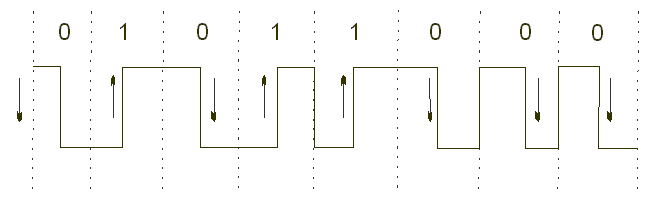
\includegraphics[width=0.5\textwidth]{pic/manchester-code.png}
\end{center}
\end{block}

\end{frame}
%--------------------------------------------------------------------------------
\begin{frame}
\frametitle{Скремблирование}
\begin{itemize}
 \item Исключающее или $Data\otimes RS$ данных с псевдослучайной последовательностью $RS$.
 \item Последовательность данных предполагается случайной и независимой от скремблирующей последовательности
\end{itemize}

\end{frame}
%--------------------------------------------------------------------------------
\begin{frame}
\frametitle{Симметричные сигналы}
\begin{itemize}
 \item Невозможно передавать составляющую постоянного тока (коаксиальный кабель)
 \item Нет смысла расходовать лишнюю энергию
 \item Использование ${\pm1}$ вместо ${0,1}$ -- биполярное кодирование
\end{itemize}
\end{frame}
%--------------------------------------------------------------------------------
%--------------------------------------------------------------------------------
\begin{frame}
\frametitle{Передача в полосе пропускания}
\begin{columns}
\column{.5\textwidth}
\begin{block}{Модуляция}
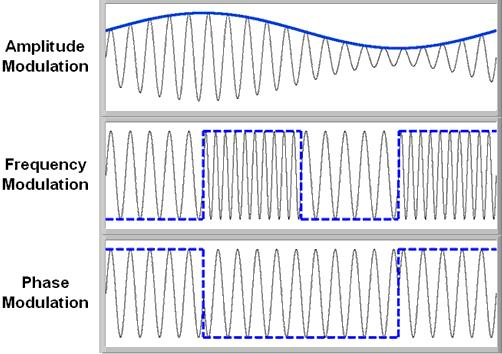
\includegraphics[width=\textwidth]{pic/modulation.jpg}
\end{block}
\column{.5\textwidth}
\begin{block}{QAM-16 с кодом Грея}
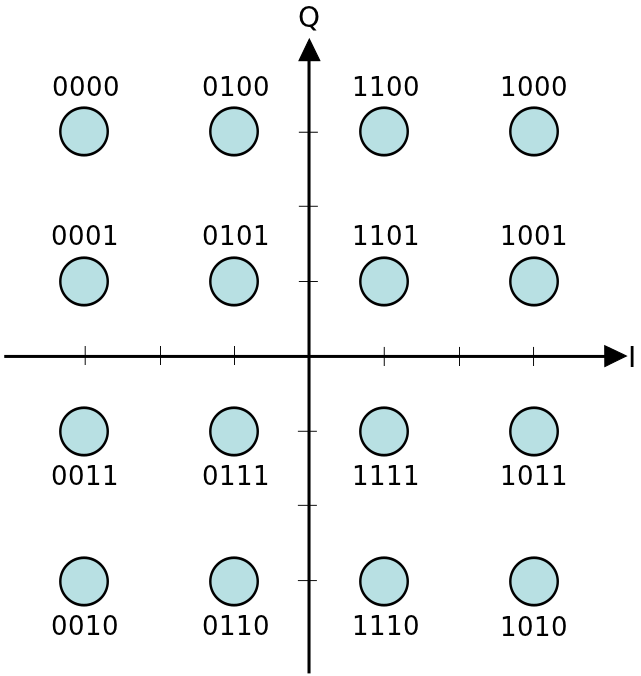
\includegraphics[width=\textwidth]{pic/16QAM_Gray_Coded.png}
\end{block}
\end{columns}
\end{frame}
%--------------------------------------------------------------------------------
\begin{frame}
\frametitle{Что такое мультиплексирование?}
\emph{Мультиплексирование} – уплотнение канала, передача данных нескольких каналов с меньшей пропускной способностью по одному каналу с большей пропускной способностью.
\begin{itemize}
	\item Частотное мультиплексирование (FDM)
	\item Ортогональное частотное мультиплексирование (OFDM)
	\item Спектральное мультиплексирование (WDM)
	\item Временное мультиплексирование (TDM)
	\item Пространственное мультиплексирование (MIMO)
	\item Мультиплексирование с кодовым разделением (CDMA)
	\item Плезиохронная цифровая иерархия (PDH)
	\item Синхронная цифровая иерархия (SDH)
\end{itemize}
\end{frame}
%--------------------------------------------------------------------------------
\begin{frame}
\frametitle{Необходимость использования мультиплексирования}
\begin{itemize}
	\item Невозможность передачи слишком коротких символов (OFDM)
	\item Независимое распространение световых волн по оптоволокну (WDM)
	\item Управление множественным доступом к одному общему каналу с высокой пропускной способностью (OFDMA, TDMA)
	\item Независимое распространение радиоволн по различным путям (MIMO)
\end{itemize}
\end{frame}
%--------------------------------------------------------------------------------
\begin{frame}
\frametitle{FDM -- частотное мультиплексирование (DSL)}
\begin{center}
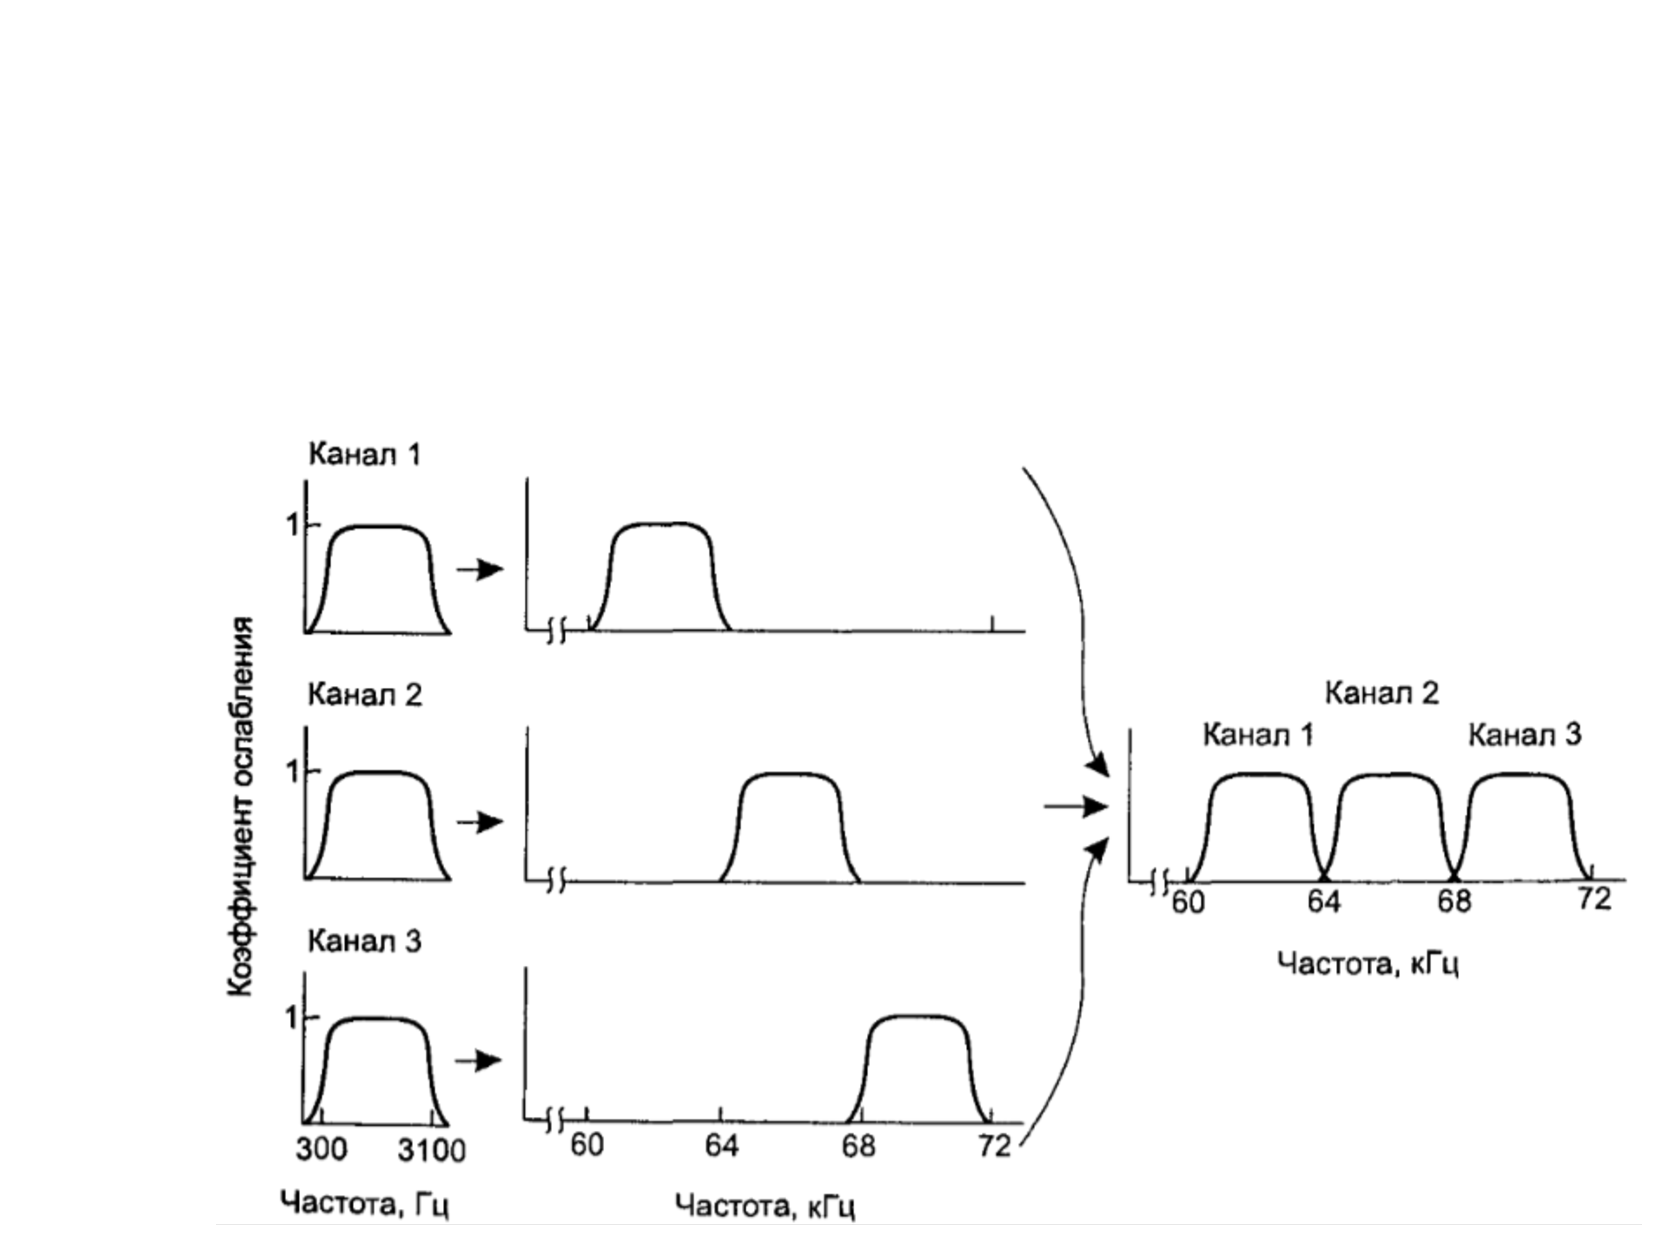
\includegraphics[width=\textwidth]{pic/fdm.pdf}
\end{center}
Нет идеальных фильтров $\Rightarrow$всегда нужно оставлять расстояние между соседними частотами
\end{frame}
%--------------------------------------------------------------------------------
\begin{frame}
\frametitle{WDM -- разделение по длине волны}
\begin{center}
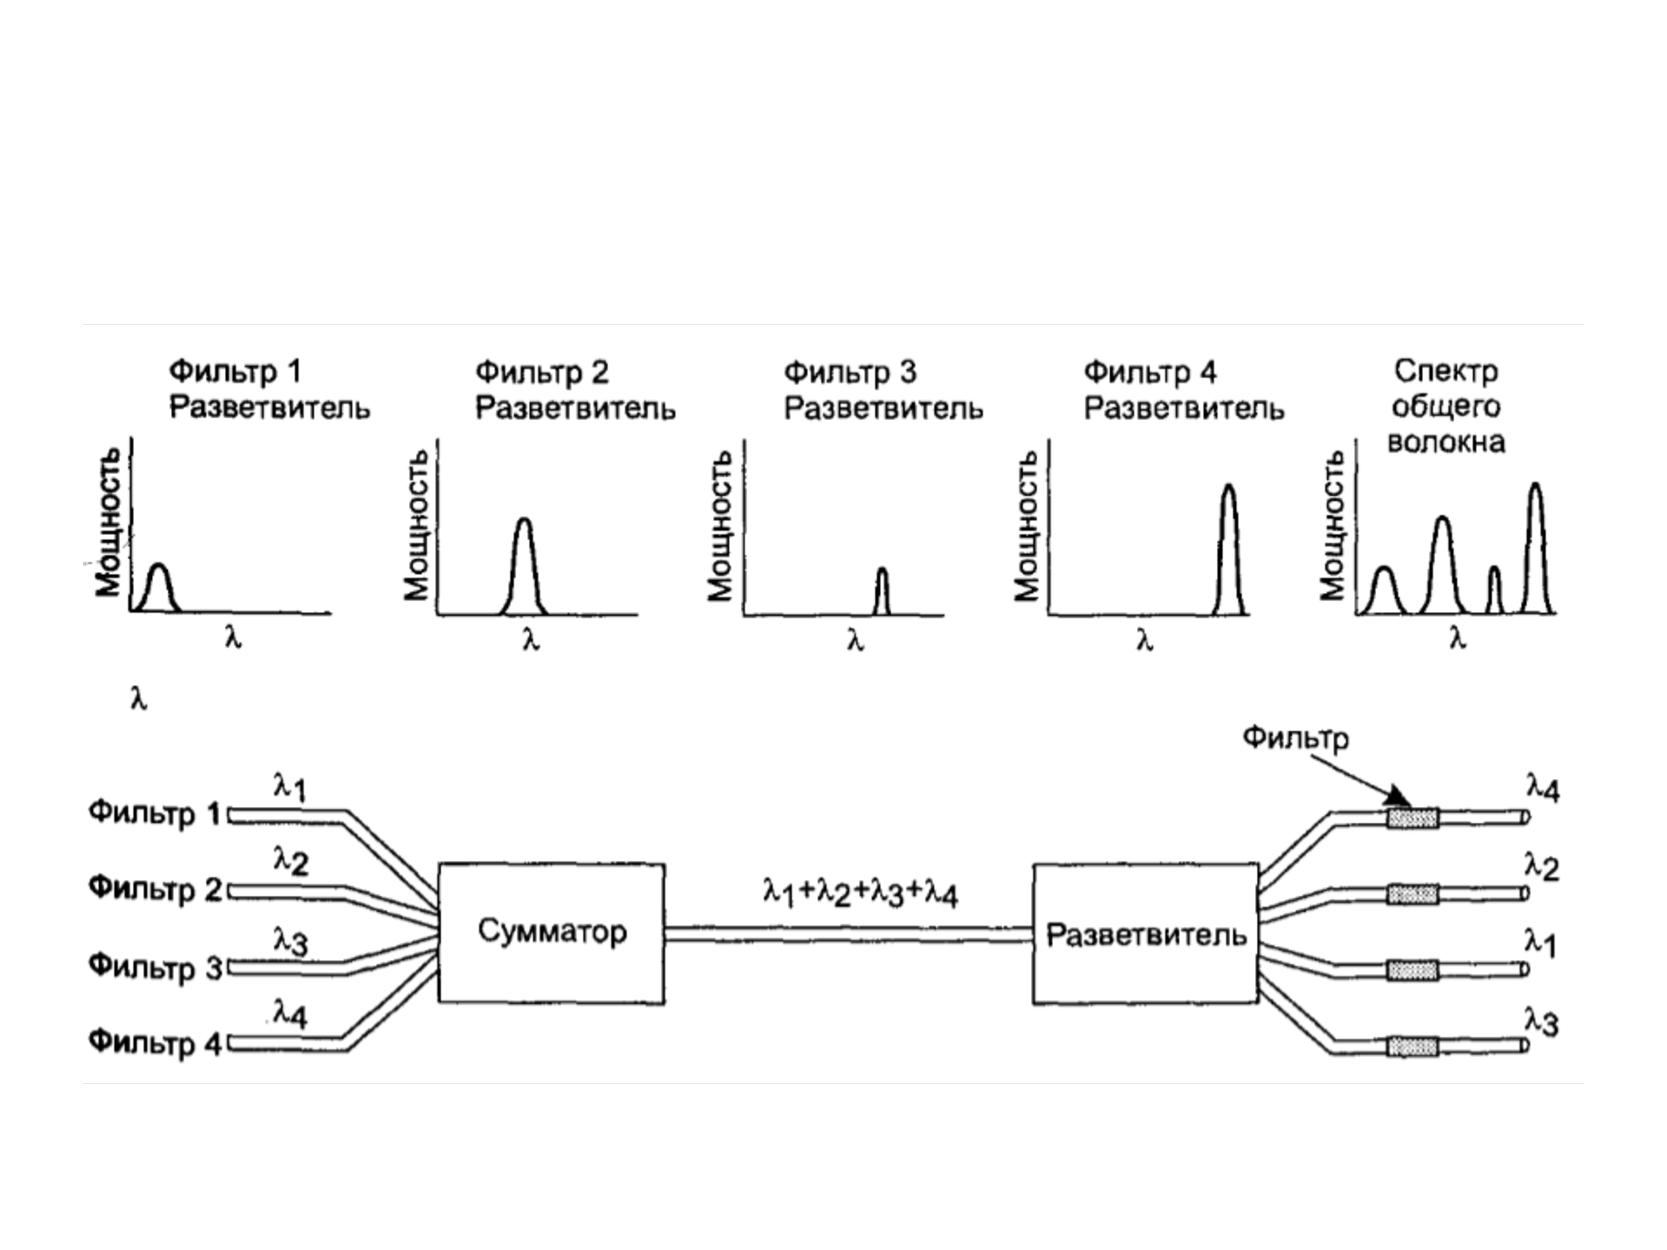
\includegraphics[width=\textwidth]{pic/wdm.pdf}
\end{center}
\end{frame}
%--------------------------------------------------------------------------------
\begin{frame}
\frametitle{Оцифровка аналоговых сигналов}
Преобразование аналогового сигнала в цифровой происходит в несколько этапов:
 \begin{itemize}
	\item Фильтрация: для голоса – 4КГц.
	\item Выборка: для 4КГц, согласно теореме Найквиста, необходимо производить 8000 измерений амплитуды (каждые 125 мкс) в секунду. В результате получается сигнал в виде амплитудно-импульсной модуляции (PAM – Pulse Amplitude Modulation)
	\item квантование -- сопоставление амплитуды дискретному количеству уровней;
	\item кодирование -- представление каждого уровня некоторым числом.
\end{itemize}
\end{frame}
%--------------------------------------------------------------------------------
\begin{frame}
\frametitle{PCM -- Pulse Code Modulation}
\begin{columns}
\column{.5\textwidth}
\begin{block}{}
\centering
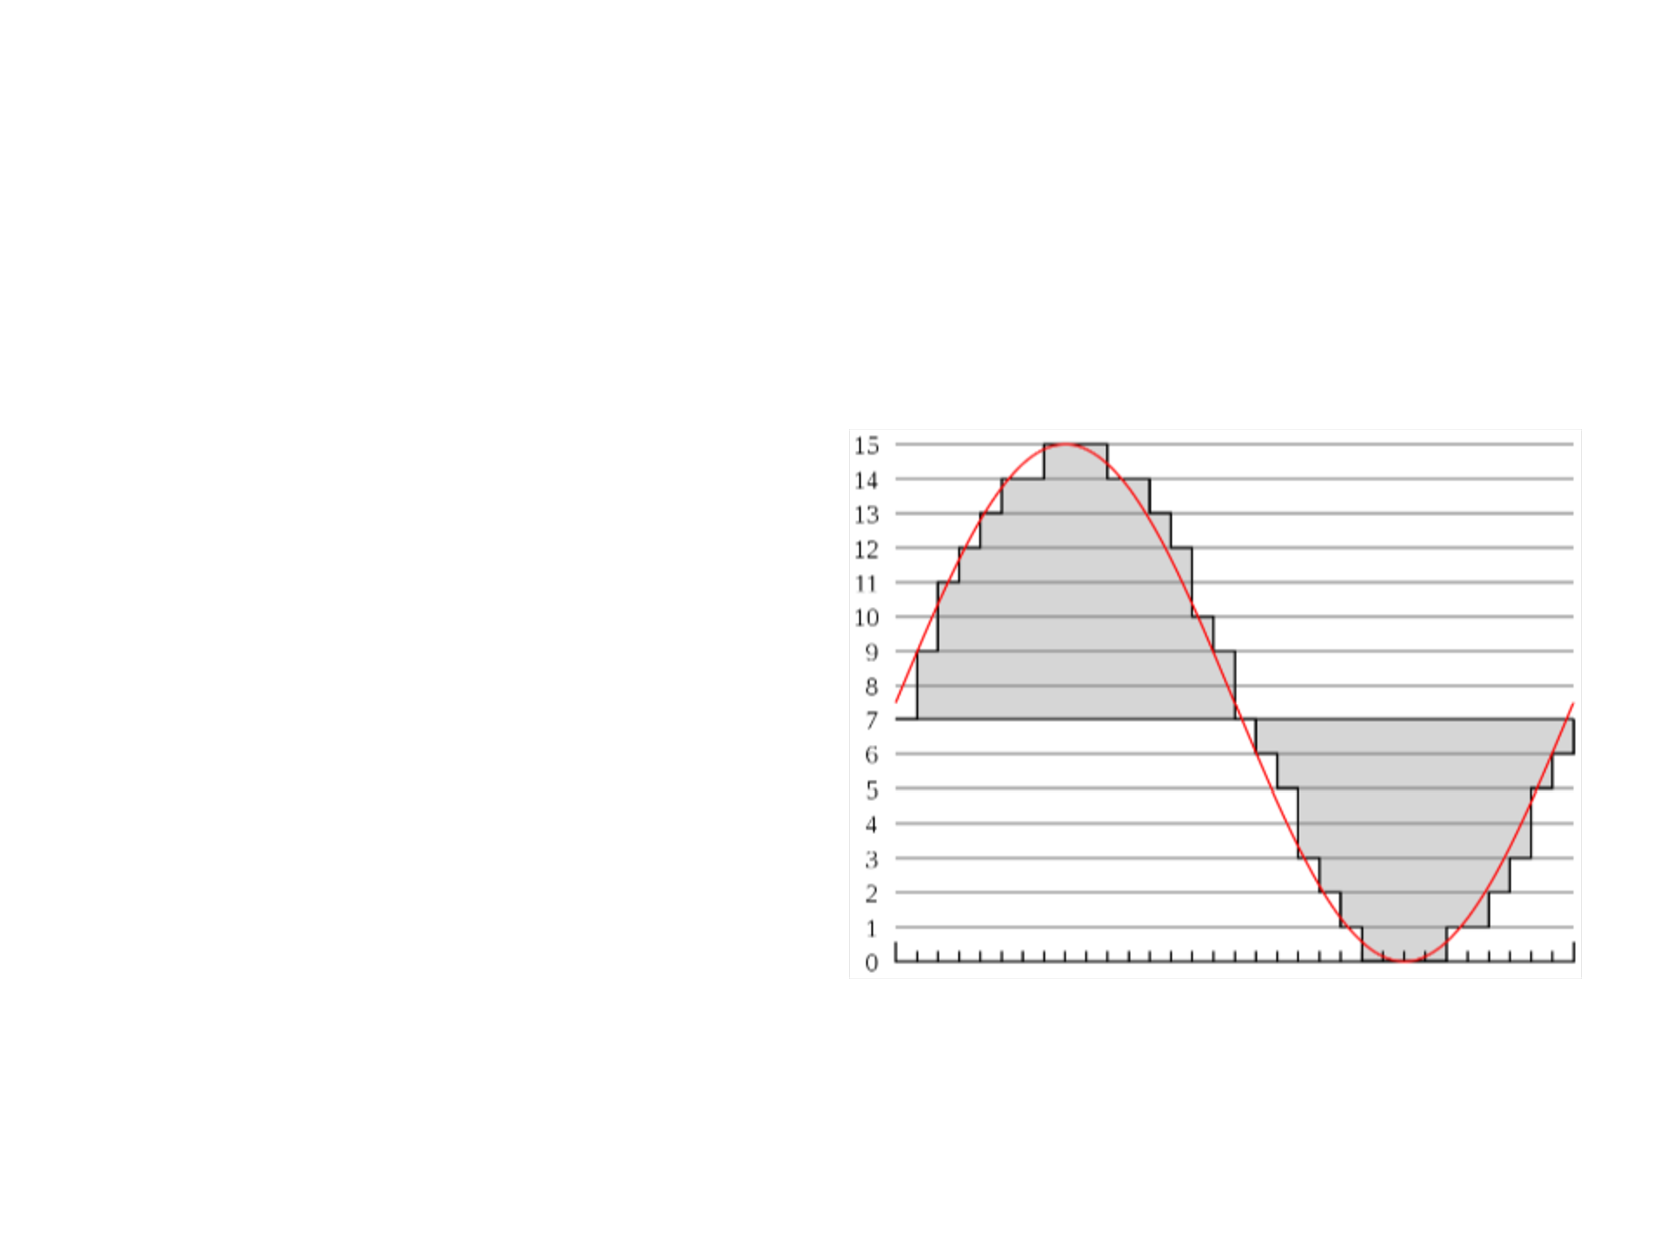
\includegraphics[width=1.1\textwidth]{pic/pcm.pdf}
\end{block}
\column{.5\textwidth}
\begin{block}{}
В результате процесса квантования, аналоговые значения амплитуды, измеренные при выборке, округляют до ближайших дискретных уровней. Как правило, для задания значения используют 8 бит, соответственно 256 дискретных значений.

В результате получается сигнал в виде импульсно-кодовой модуляции (PCM – Pulse Code Modulation).
\end{block}
\end{columns}
\end{frame}
%--------------------------------------------------------------------------------
\begin{frame}
\frametitle{PCM -- Pulse Code Modulation}
\begin{columns}
\column{.35\textwidth}
\begin{block}{}
\centering
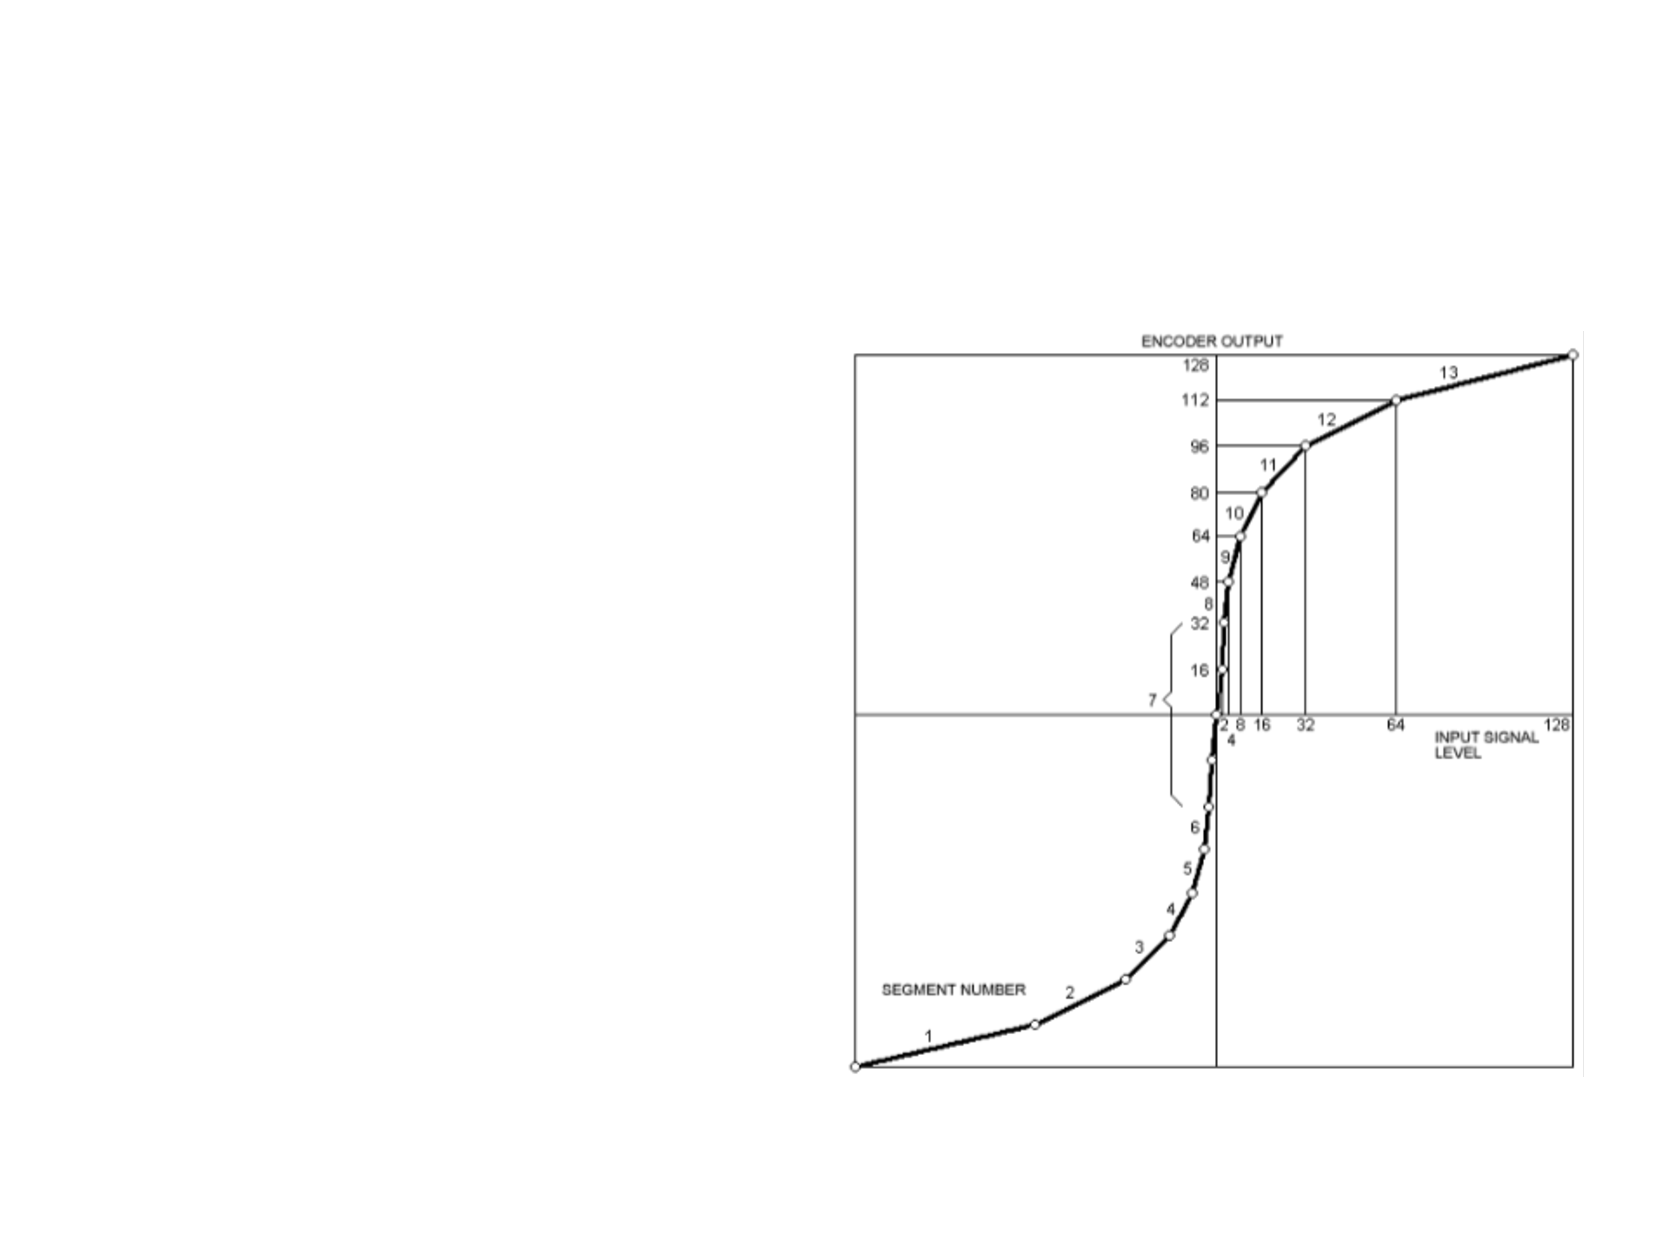
\includegraphics[width=1.1\textwidth]{pic/pcm-2.pdf}
\end{block}
\column{.65\textwidth}
\begin{block}{}
За счёт конечного числа уровней, при дискретизации возникает ошибка дискретизации.

Компандирование – увеличение числа шагов квантования в области малых значений амплитуды входного сигнала.

A-law algorithm:
\begin{displaymath}
F(x) = sgn(x) \left\{ \begin{array}{ll}
\frac{A |x|}{1 + \log (A)}, & |x| < A\\
\frac{1 + \log (A |x|)}{1 + \log (A)}, & \frac{1}{A} < x < 1\\
\end{array} \right.
\end{displaymath}
\end{block}
\end{columns}
\end{frame}
%--------------------------------------------------------------------------------
\begin{frame}
\frametitle{Основной цифровой канал - ОЦК}
\begin{itemize}
	\item Основной цифровой канал (DS0 – Digital Signal 0 или E0) – 64 Кбит/c канал, изначально использовался для передачи оцифрованного голоса, скорость получается из 8000 отсчётов в секунду и 8 бит ИКМ (PCM) на каждый отсчёт.
	\item В настоящее время – основной канал мультиплексирования в Плезиохронная цифровой иерархии.
\end{itemize}
\end{frame}
%--------------------------------------------------------------------------------
\begin{frame}
\frametitle{Плезиохронная цифровая иерархия}
Плезиохронная цифровая иерархия (PDH - Plesiochronous Digital Hierarchy) – телекоммуникационная технология предназначенная для передачи голоса и данных в цифровом виде, основанная на временном мультиплексировании ОЦК.
\begin{center}
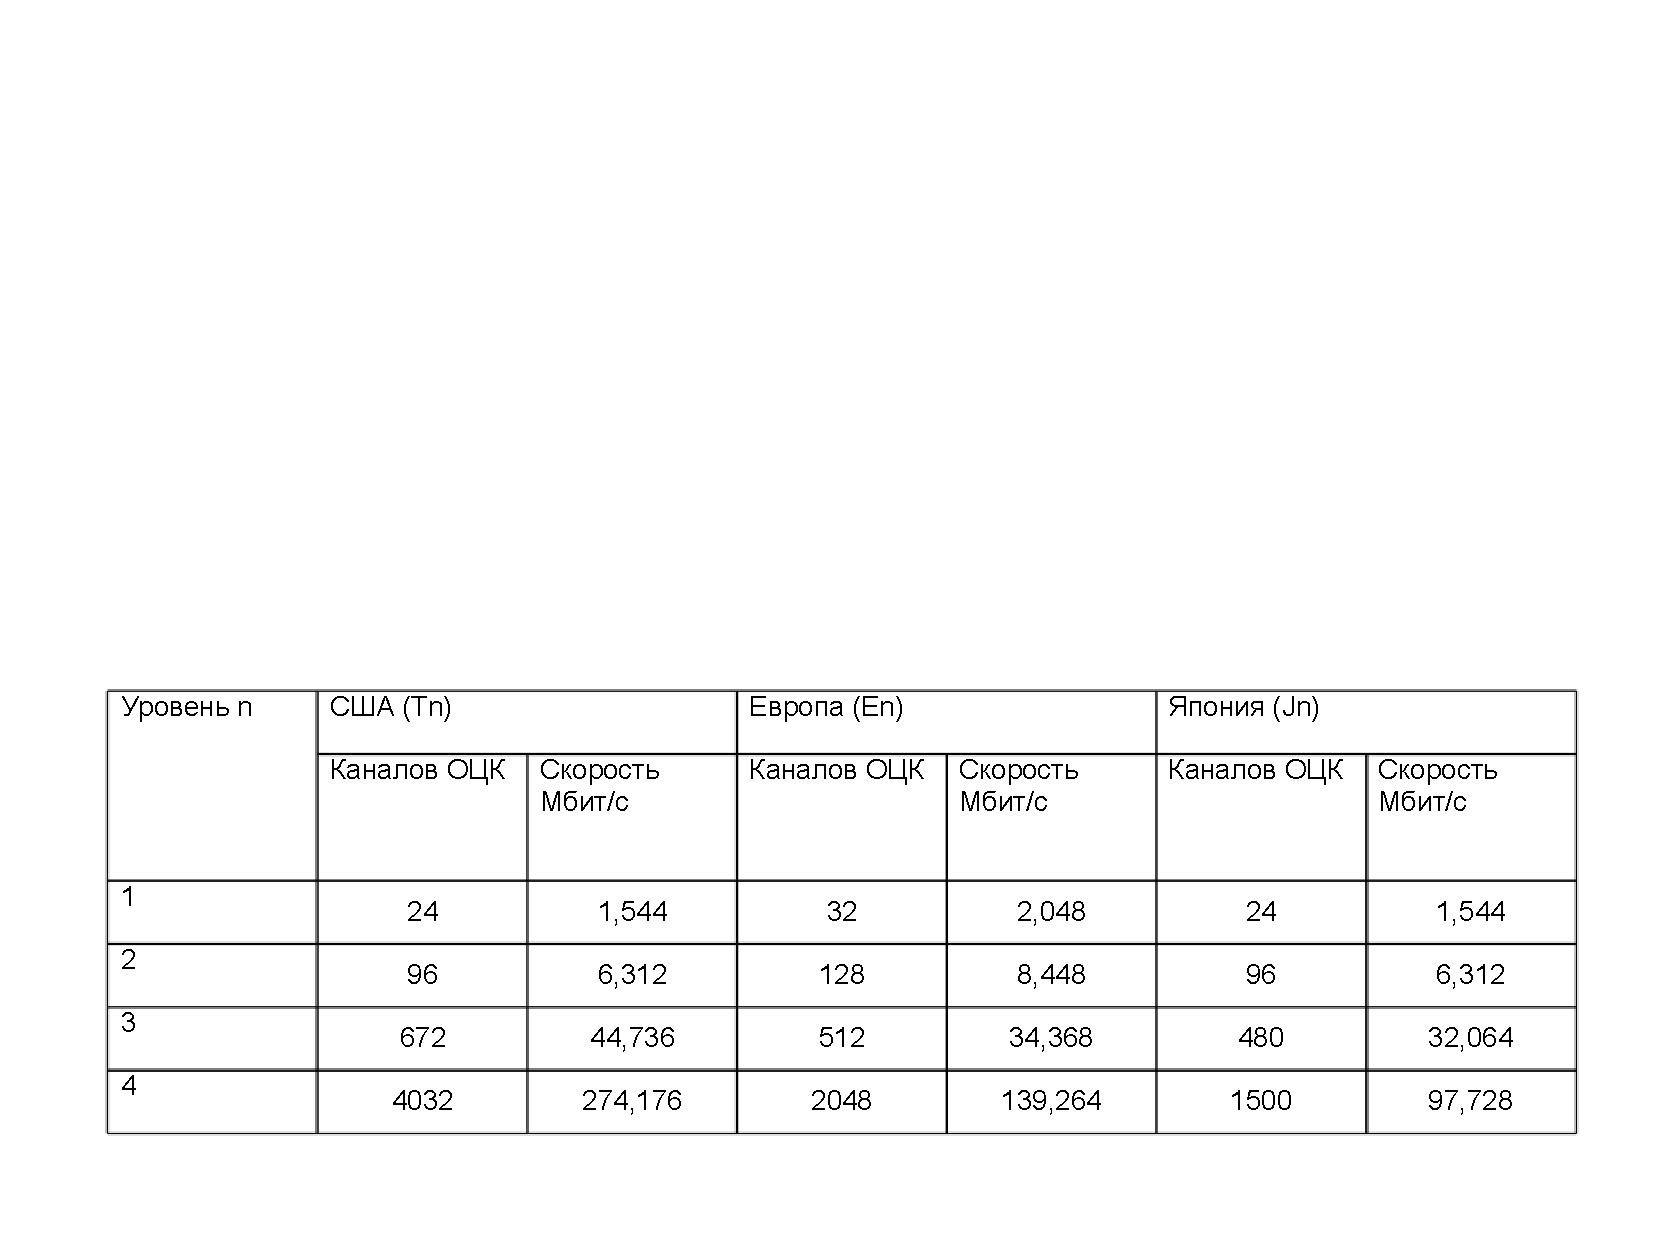
\includegraphics[width=\textwidth]{pic/pdh.pdf}
\end{center}
\end{frame}
%--------------------------------------------------------------------------------
\begin{frame}
\frametitle{Структура кадра E1}
\begin{center}
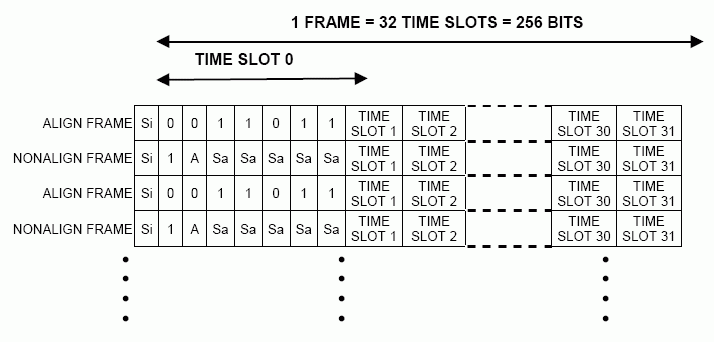
\includegraphics[width=\textwidth]{pic/e1.png}
\end{center}
\end{frame}
%--------------------------------------------------------------------------------
\begin{frame}
\frametitle{Синхронная цифровая иерархия}
Синхронная цифровая иерархия (SDH - Synchronous Digital Hierarchy) – современная телекоммуникационная, использующая согласованную синхронизацию, технология предназначенная для передачи цифровых потоков данных. В основе – временное мультиплексирование синхронных транспортных модулей STM-1. Скорость уровня 1 - 155,52 МБит/c
\end{frame}
%--------------------------------------------------------------------------------
\begin{frame}
\frametitle{Структура кадра STM-1}
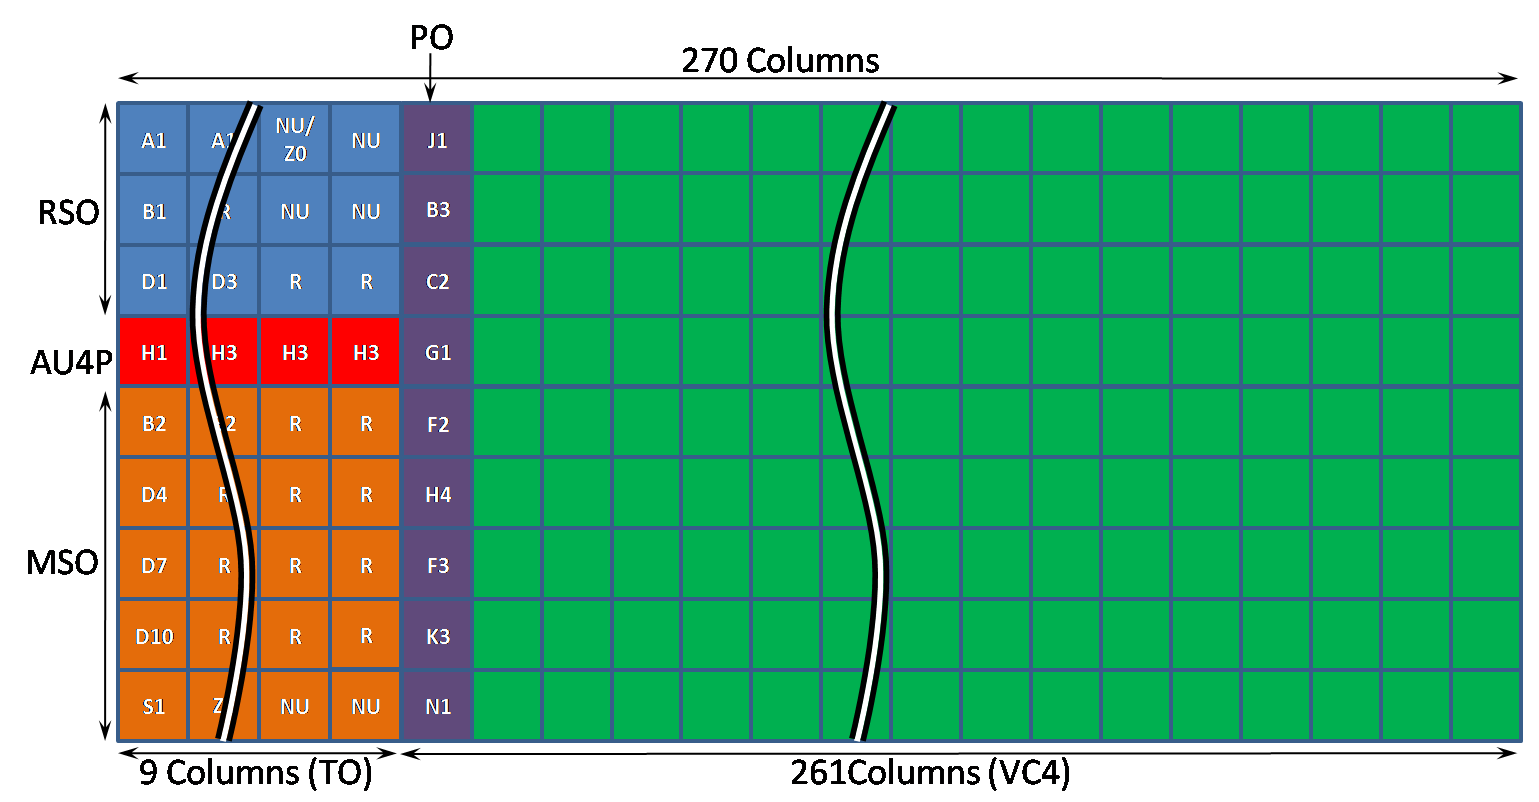
\includegraphics[width=\textwidth]{pic/stm-1.png}
\end{frame}
%--------------------------------------------------------------------------------
\begin{frame}
\frametitle{Мультиплексирование в беспроводных сетях}
\begin{itemize}
	\item OFDM -- Orthogonal Frequency Division Multiplexing (IEEE 802.11 DVB, DAB)
	\item OFDMA -- Orthogonal Frequency Division Multiple Access (IEEE 802.16, LTE)
	\item SDMA -- Spatial Division Multiple Access (IEEE 802.11n, LTE) based on MIMO
	\item CDMA -- Code Division Multiple Access (CDMA-2000 3G)
\end{itemize}
Необходимость мультиплексирования обусловлена сложным поведением канала передачи и необходимостью множественного доступа в сотовых сетях связи
\end{frame}
%--------------------------------------------------------------------------------
\begin{frame}
\frametitle{OFDM}
\begin{itemize}
	\item Эффективное использование полосы пропускания.
	\item Генерация символов со скоростью Найквиста
	\item Соседние поднесущие взаимно ортогональны
\end{itemize}
$$
\textrm{Baseband Signal:} 
\sum_{i=-N}^{N}a_i \cdot sin(2\pi \cdot i \cdot \omega_0),
$$
$$
\omega_0 = \frac{2 \pi}{ T}, T \textrm{ -- длительность символа}
$$
Эффективная реализация стала возможной только благодаря использованию ДПФ
\end{frame}
%--------------------------------------------------------------------------------
\begin{frame}
\frametitle{От интеграла Фурье к ДПФ}
Интеграл Фурье --  спектр непрерывного сигнала:
$$
F(f) = \frac{1}{\sqrt{2 \pi}}\int_{-\infty}^{\infty}\nu(t)\cdot e^{-j\cdot 2\pi \omega t}d\omega
$$
Дискретное по времени преобразование Фурье -- спектр дискретизованного сигнала:
$$
X_D(f) = \Delta t \sum_{k=-\infty}^{\infty}x(k\Delta t) e ^{-j \cdot 2 \pi f k \Delta t}
$$
$$
x(k\Delta t) = \int_{-\frac{f_D}{2}}^{\frac{f_D}{2}}X_D(f) e ^{-j \cdot 2 \pi f k \Delta t} df
$$
\end{frame}
%--------------------------------------------------------------------------------
\begin{frame}
\frametitle{Дискретное Преобразование Фурье}
ДПФ -- спектр периодического дискретизованного сигнала
$$
X_k = \sum_{n=0}^{N-1}x_n \cdot e^{\frac{-2\pi \cdot j}{N}k n}
$$
$$
x_n = \frac{1}{N}\sum_{n=0}^{N-1}X_k\cdot e^{\frac{2\pi \cdot j}{N}k n}
$$
Доказательство:
$$
x(t) = \sum_{k=-\infty}^{\infty}c_k \cdot e^{i \omega_k t} \textrm{ -- спектр периодического сигнала}
$$
$$
x(t_n) = \sum_{k=-\infty}^{\infty}c_k \cdot e^{j \omega_k t_n} = \sum_{k=-\infty}^{\infty}c_k \cdot e^{\frac{2\pi \cdot j}{N}k n} = 
 \sum_{k=0}^{N-1}X_k \cdot e^{\frac{2\pi \cdot j}{N}k n}
$$
$$
t_n = \frac{n}{N}T,
e^{\frac{2\pi j}{N} (k + mN)n} = e^{\frac{2\pi \cdot j}{N}k n},
X_K = \sum_{l = -\infty}^{\infty}c_{k+lN}
$$
\end{frame}
%--------------------------------------------------------------------------------
\begin{frame}
\frametitle{Свойства ДПФ}

Первая половина отсчётов в частотной области -- положительные частоты по возрастанию ($0 \ldots \frac{f_D}{2}$).
Вторая половина отсчётов - отрицательные частоты по возрастанию ($-\frac{f_D}{2}\ldots 0$).
\begin{columns}
\column{.5\textwidth}
\begin{block}{}
\centering
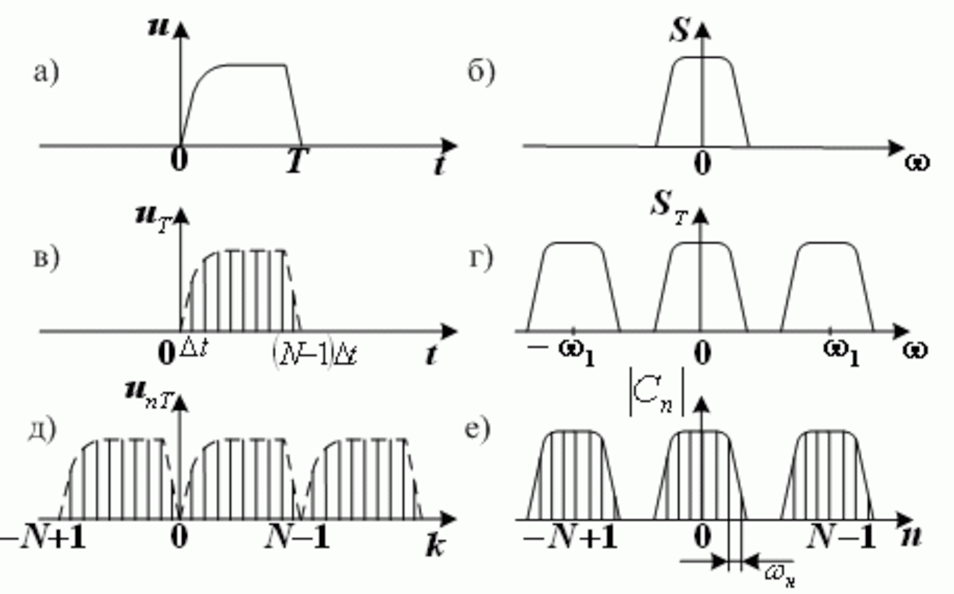
\includegraphics[width=\textwidth]{pic/dft.pdf}
\end{block}
\column{.5\textwidth}
\begin{block}{ДПФ в матричном виде}
$$
\overline{X} = A\cdot \overline{x}
$$
$$
A_{mn} =
exp \Big(
-2\pi j \frac{(m-1)(n - 1)}{N}
\Big)
$$
\end{block}
\end{columns}
Если N является степенью двойки -- то возможно эффективное вычисление ДПФ со сложностью $O (N \log N)$
\end{frame}
%--------------------------------------------------------------------------------
\begin{frame}
\frametitle{Передача  OFDM сигнала в идеальном канале}
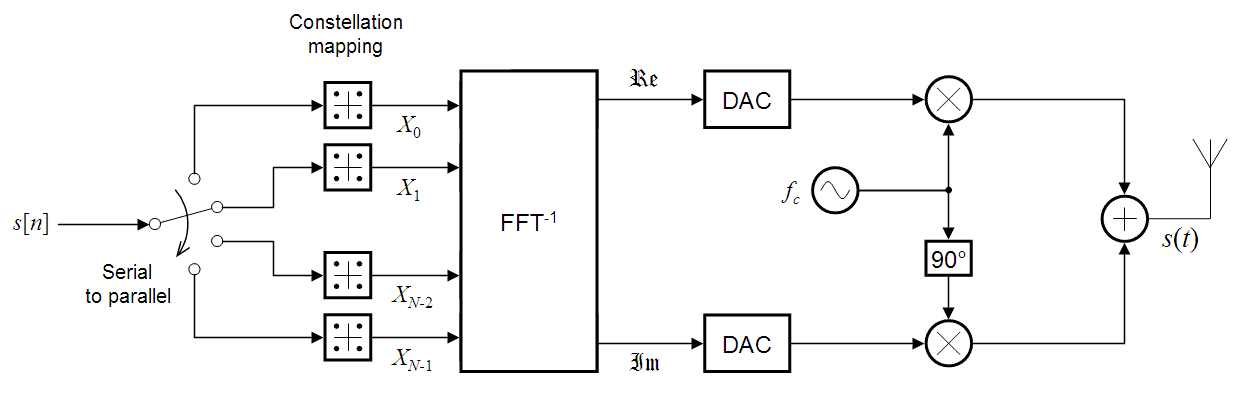
\includegraphics[width=\textwidth]{pic/OFDM_transmitter_ideal.png}
\end{frame}
%--------------------------------------------------------------------------------
\begin{frame}
\frametitle{Простейший пример OFDM с тремя поднесущими (R) в
комплексной области}
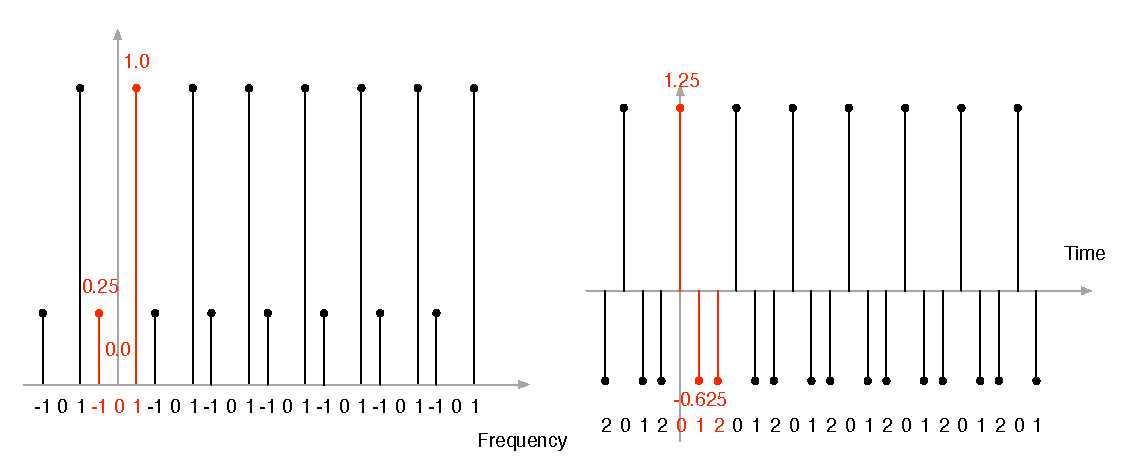
\includegraphics[width=\textwidth]{pic/fft-example.pdf}
\begin{itemize}
  \item Амплитудная модуляция на каждой поднесущей ($f_{-1}, f_0, f_1$)
  \item Пусть на отрицательной частоте передаем 0.25, а на положительной -- 1, то есть 
  $$
  f(t) = 0.25 \cdot e^{-j\omega t} + 0 + 1.0\cdot e^{j\omega t} , \omega = \frac{2\pi}{3}, \Delta T = 1
  $$
  $$
  0.25 \textrm{ -- коэффициент АМ для } f_{-1}, 0\textrm{ -- для } f_0, 1\textrm{ -- для }  f_1
  $$
\end{itemize}
\end{frame}
%--------------------------------------------------------------------------------
\begin{frame}[fragile]
\frametitle{Простейший пример OFDM с тремя поднесущими (R)}

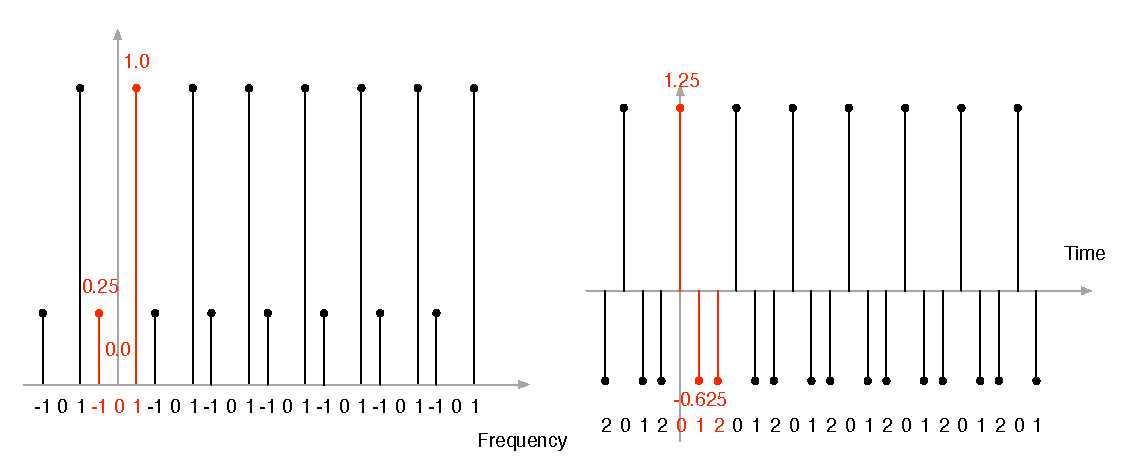
\includegraphics[width=\textwidth]{pic/fft-example.pdf}
\newline
\tiny
Не будем использовать циклический префикс, то есть во временной области имеем 3 отсчёта: $0, 1, 2$.
\begin{verbatim}
> x<-0:2 # 3 поднесущих в частотной области дадут 3 временных отсчёта с номерами $0, 1, 2$
> x
[1] 0 1 2
\end{verbatim}
3 отсчёта в частотной области ($0, 1, 2=-1$) -- это коэффициенты соответствующих ортогональных синусоид:
\begin{verbatim}
> 0 + 1 * exp (complex (re=0, im=(2*pi/3*x))) + 0.25 * exp (complex (re=0, im=(-2*pi/3*x)))
[1]  1.250+0.0000000i -0.625+0.6495191i -0.625-0.6495191i
> fft (c (0, 1, 0.25), inverse=T) # Получим те же самые коэффициенты с помощью обратного ДПФ
[1]  1.250+0.0000000i -0.625+0.6495191i -0.625-0.6495191i
\end{verbatim}
В действительной области $e^{-j\omega t}$ и $e^{j\omega t} $ ``неразличимы''
\end{frame}
%--------------------------------------------------------------------------------
\begin{frame}
\frametitle{Приём OFDM сигнала в идеальном канале}
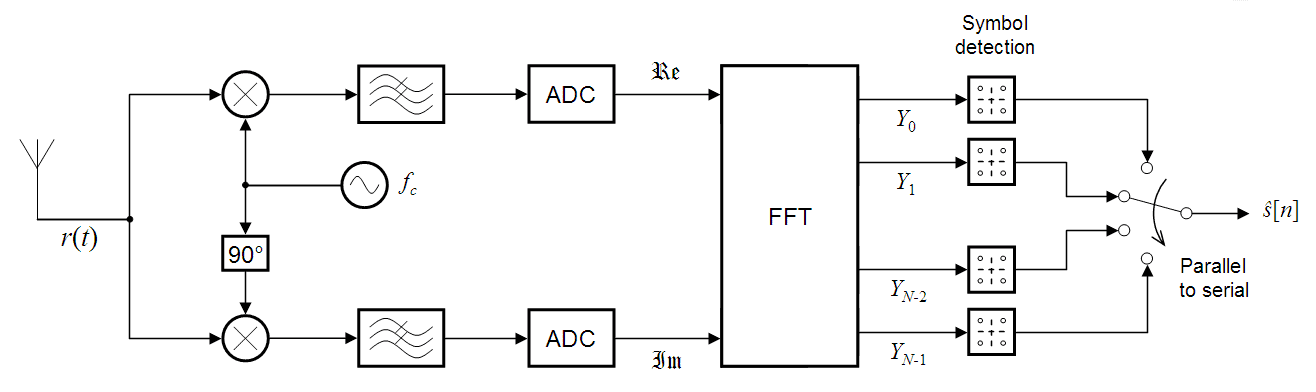
\includegraphics[width=\textwidth]{pic/OFDM_receiver_ideal.png}
\newline
Циклическая свёртка во временной области ведет к перемножению спектра в частотной:
$$
 y(t) = x(t)\otimes h(t) \Rightarrow Y(f) = H(f)\cdot X(f)
$$
При наличии импульсной характеристики канала нужно только умножение в частотной области!

Межсимвольная интерференция?
\end{frame}
%--------------------------------------------------------------------------------
\begin{frame}
\frametitle{Многолучевое распространение -- межсимвольная интерференция}
\begin{center}
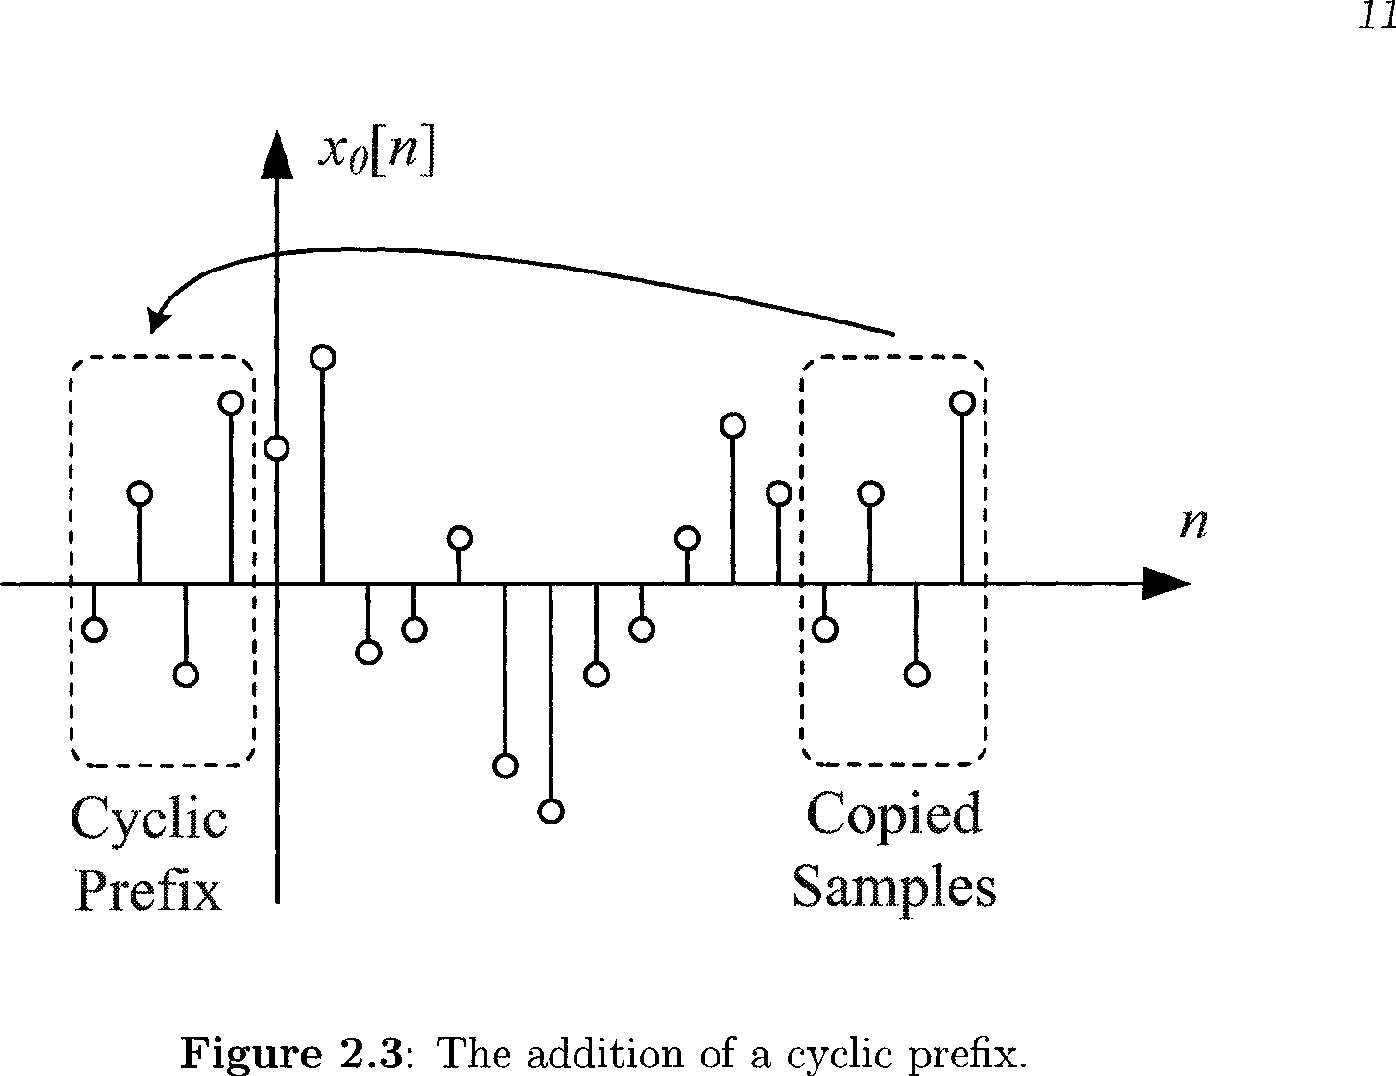
\includegraphics[width=0.8\textwidth]{pic/cyclic-prefix.png}
\end{center}
Циклический префикс > импульсной характеристики канала!
\end{frame}
%--------------------------------------------------------------------------------
\begin{frame}
\frametitle{Особенности OFDM}

Нужно точно знать импульсную характеристику канала.
$$
 y(t) = x(t)\otimes h(t) \Rightarrow Y(f) = H(f)\cdot X(f)
$$
Необходима точная синхронизация по частоте
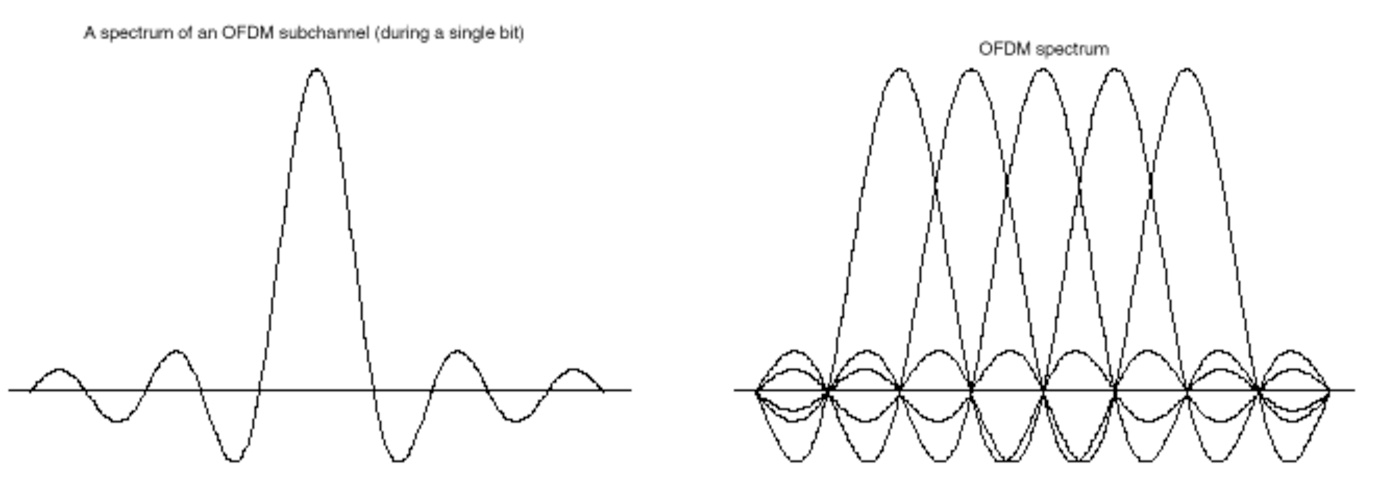
\includegraphics[width=0.4\textwidth]{pic/ofdm-spectrum.pdf}

Высокий коэффициент линейности принимающего фильтра
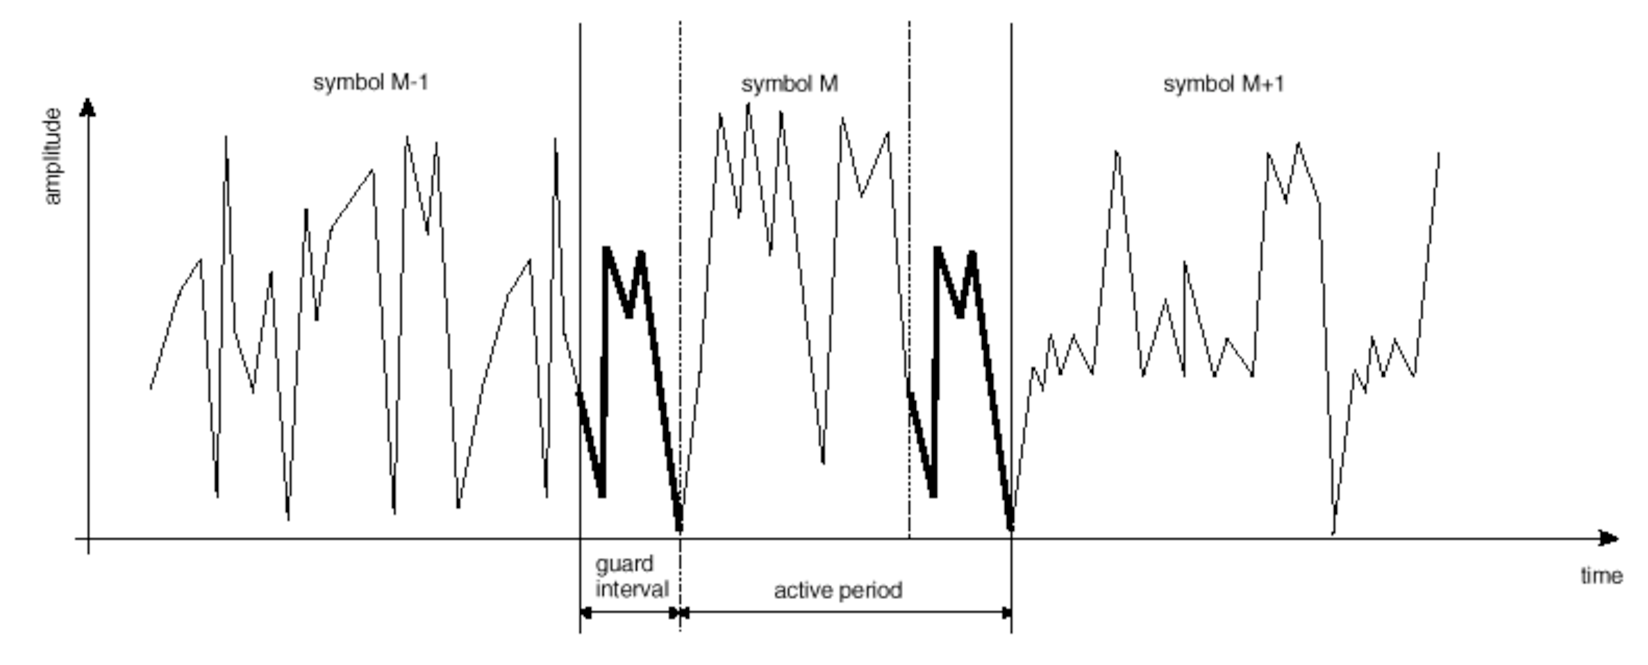
\includegraphics[width=0.8\textwidth]{pic/ofdm-linearity.pdf}
\end{frame}
%--------------------------------------------------------------------------------
\begin{frame}
\frametitle{Наличие преамбулы, опорных символов, пилотных поднесущих}
\begin{center}
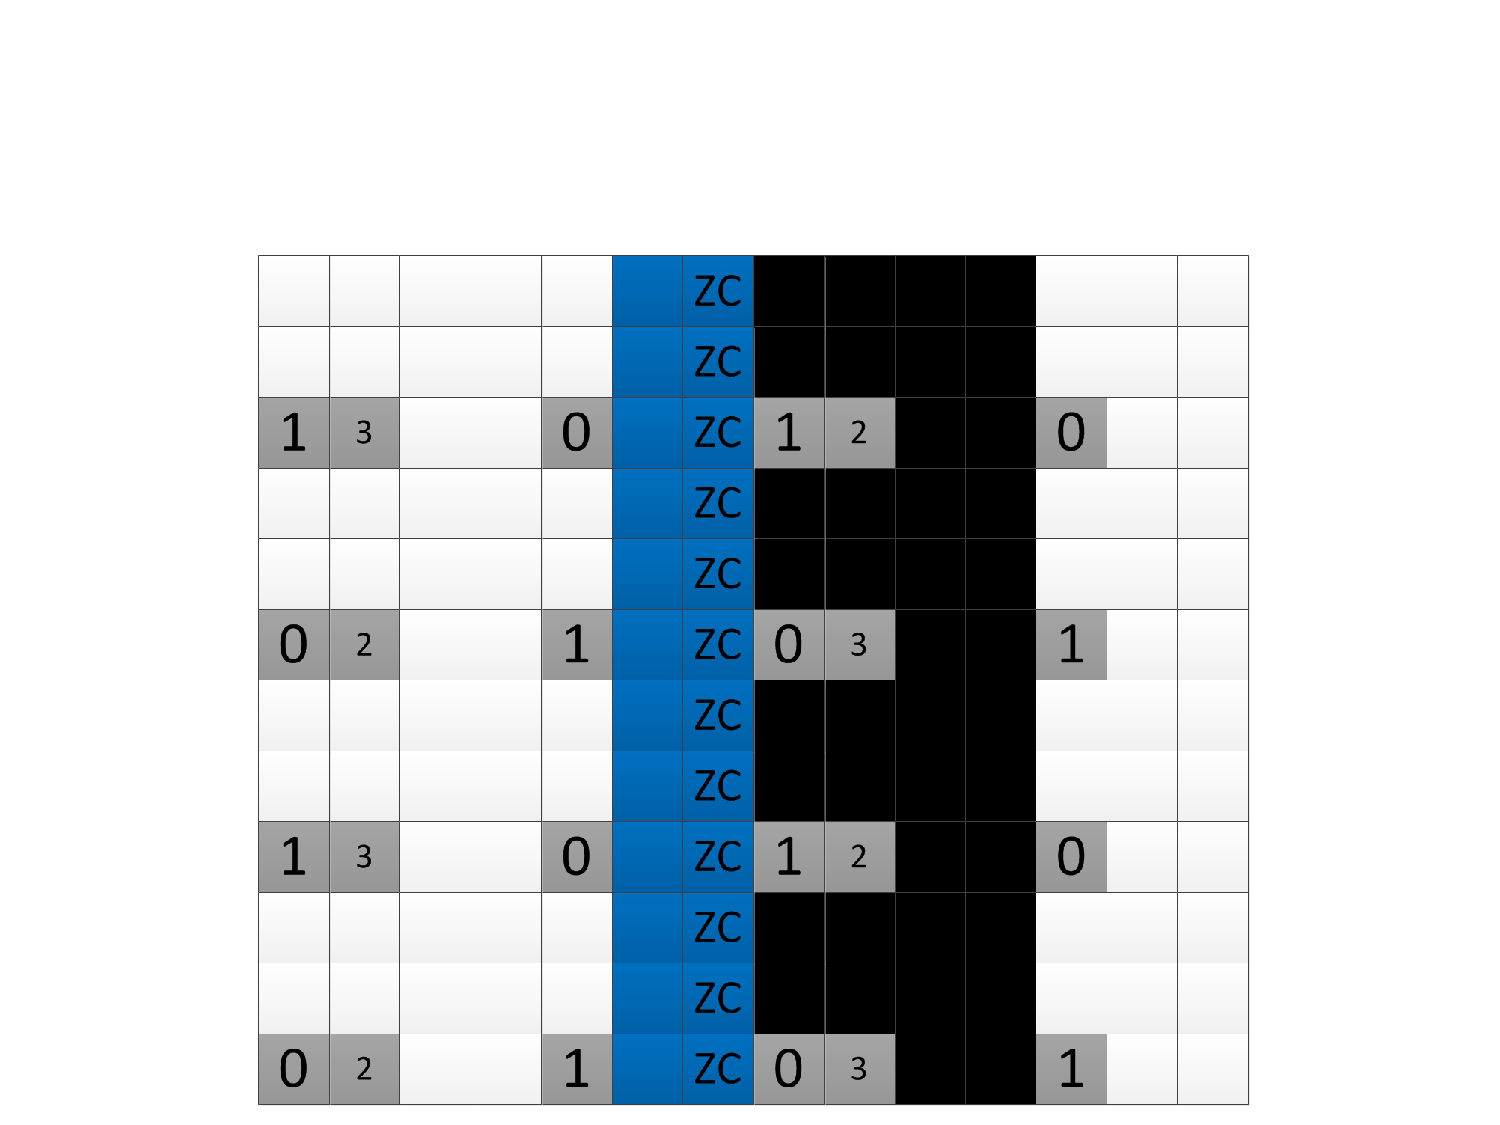
\includegraphics[width=0.6\textwidth]{pic/lte-DL.pdf}
\end{center}
Нужно помнить о частоте и времени когерентности канала!
\end{frame}
%--------------------------------------------------------------------------------
\begin{frame}
\frametitle{MIMO -- Multiple Output Multiple Input}
Можно ли ``нажиться'' на многолучевом распространении?
\begin{center}
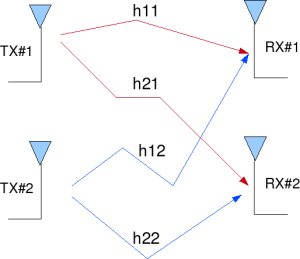
\includegraphics[width=0.25\textwidth]{pic/2tx_2rx_mimo.png}
\end{center}
$$
\mathbf{H} =
\left(
\begin{array}{cc}
h_{11} & h_{12} \\
h_{21} & h_{22}
\end{array}
\right),
\mathbf{x} =
\left(
\begin{array}{c}
x_{1} \\ x_{2}
\end{array}
\right),
\mathbf{y} = \mathbf{H}\cdot \mathbf{x}
$$
\begin{itemize}
	\item Выбрать символы для передачи.
	\item Подобрать комплексные коэффициенты усиления сигнала, передаваемого с каждой из антенн
	\item Выбрать мощность передачи на каждой из антенн
\end{itemize}
\end{frame}
%--------------------------------------------------------------------------------
\begin{frame}
\frametitle{MIMO}
\begin{center}
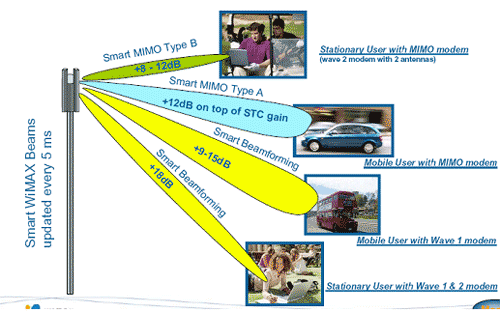
\includegraphics[width=0.5\textwidth]{pic/MAS_gains.png}
\end{center}
\begin{itemize}
	\item Координация интерференции
	\item Снижение негативного воздействия многолучевых замираний
	\item Пространственное разделение пользователей
\end{itemize}
Как точно оценивать канал?
\end{frame}
%--------------------------------------------------------------------------------
\begin{frame}
\frametitle{Численный пример: $3\times3$ MIMO  в сотовых сетях}
\begin{center}
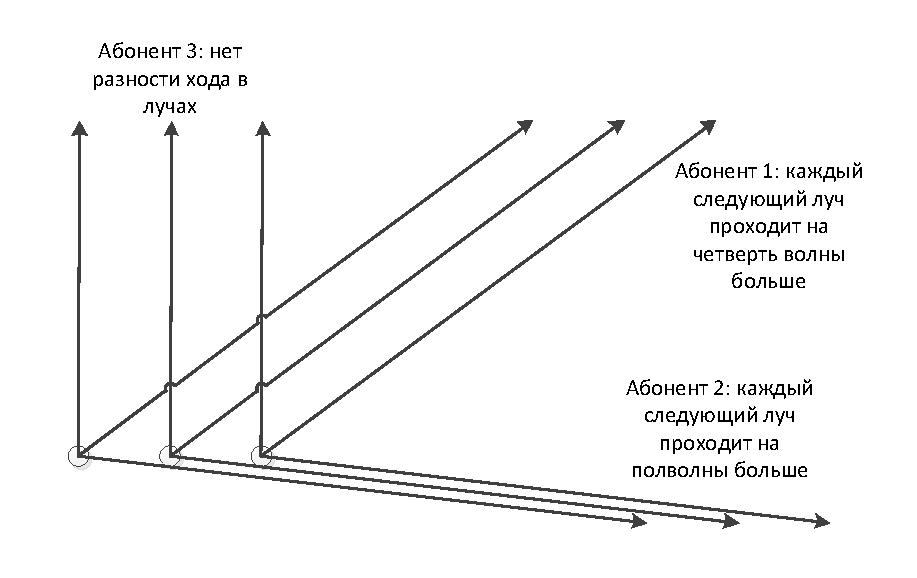
\includegraphics[width=0.6\textwidth]{pic/MIMO-example.pdf}
\end{center}
$$
\mathbf{H} =
\left(
\begin{array}{ccc}
1 & e^{j\frac{\pi}{2}} & e^{j\pi}\\
1 & e^{j\pi}           & 1       \\
1 &  1                 & 1       \\
\end{array}
\right),
\mathbf{y_p} = \mathbf{H}\cdot \mathbf{x_p}
$$
\begin{center}
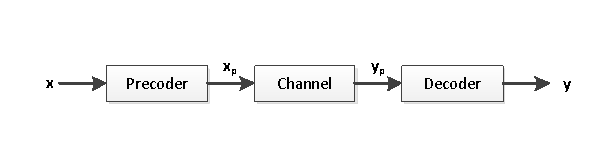
\includegraphics[width=\textwidth]{pic/MIMO-precoder.pdf}
\end{center}
\end{frame}
%--------------------------------------------------------------------------------
\begin{frame}
\frametitle{Численный пример: $3\times3$ MIMO  в сотовых сетях}
\begin{center}
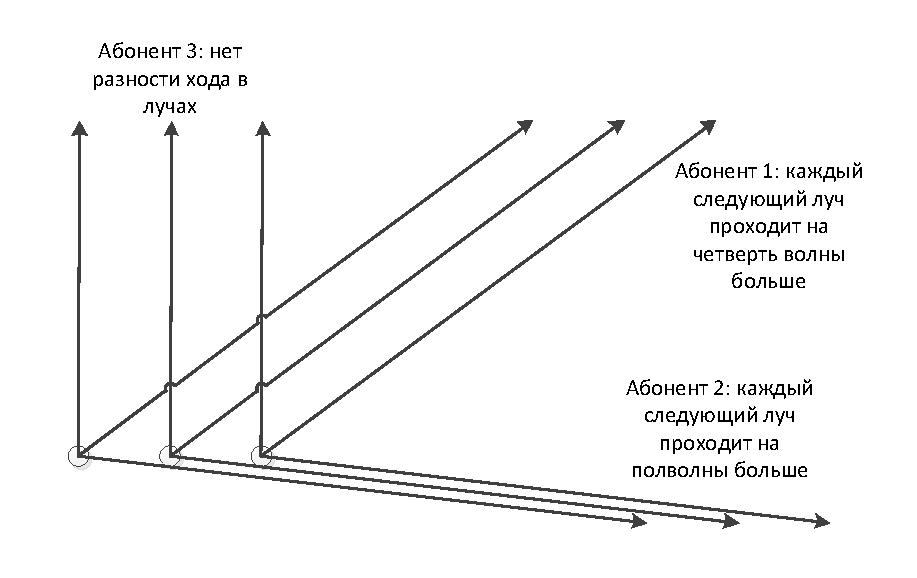
\includegraphics[width=0.6\textwidth]{pic/MIMO-example.pdf}
\end{center}
$$
\mathbf{H} =
\left(
\begin{array}{ccc}
1 & e^{j\frac{\pi}{2}} & e^{j\pi}\\
1 & e^{j\pi}           & 1       \\
1 &  1                 & 1       \\
\end{array}
\right),
\mathbf{x} =
\left(
\begin{array}{c}
1 \\ -1 \\ 0.5 \\
\end{array}
\right)
$$
Каждому абоненту передаем символ $\mathbf{x}_i, i=\{1,2,3\}$.

$\mathbf{y}_i, i=\{1,2,3\}$ -- декодированный сигнал, принятый $i$-м абонентом. Как сделать $\mathbf{y}_i = \mathbf{x}_i$?
\end{frame}
%--------------------------------------------------------------------------------
\begin{frame}[fragile]
\frametitle{Построение матрицы передаточных характеристик канала (R)}
$$
\mathbf{H} =
\left(
\begin{array}{ccc}
1 & e^{j\frac{\pi}{2}} & e^{j\pi}\\
1 & e^{j\pi}           & 1       \\
1 &  1                 & 1       \\
\end{array}
\right)
$$
{
\tiny
\begin{verbatim}
> channel<-matrix (c(1, 1, 1,
+ exp (complex (re=0, im=pi/2)),exp (complex (re=0, im=pi)), 1,
+ exp (complex (re=0, im=pi)), 1,1),
+ ncol=3)
> channel
     [,1]  [,2]  [,3]
[1,] 1+0i  0+1i -1+0i
[2,] 1+0i -1+0i  1+0i
[3,] 1+0i  1+0i  1+0i
\end{verbatim}
}
\end{frame}
%--------------------------------------------------------------------------------
\begin{frame}[fragile]
\frametitle{Сингулярное разложение матрицы $\mathbf{H} = \mathbf{U} \mathbf{D} \mathbf {V}^{H}$}
{
\tiny
\begin{verbatim}
> svd(channel)
$d
[1] 2 2 1

$u
                      [,1]                  [,2]                 [,3]
[1,] -0.4082483-0.0000000i  0.2357023-0.6666667i 0.5773503-0.0000000i
[2,] -0.6123724-0.2041241i  0.2154822+0.4511845i 0.0000000-0.5773503i
[3,] -0.6123724+0.2041241i -0.4511845+0.2154822i 0.0000000+0.5773503i

$v
                      [,1]                  [,2]                  [,3]
[1,] -0.8164966+0.0000000i  0.0000000+0.0000000i  0.5773503+0.0000000i
[2,]  0.0000000+0.4082483i -0.6666667-0.2357023i  0.0000000+0.5773503i
[3,] -0.4082483+0.0000000i -0.2357023+0.6666667i -0.5773503+0.0000000i

>
\end{verbatim}
}
\begin{itemize}
  \item Передаваемые базовой станцией символы: $\mathbf{x}$
  \item Передаваемые с антенн символы: 
  $
  \mathbf{x_p} = \mathbf {V} \mathbf {x}
  $
  \item Принимаемые на антеннах получателей символы:
  $
  \mathbf{y_p} = \mathbf{H}\cdot \mathbf{x_p} = \mathbf{U} \mathbf{D} \mathbf {V}^{H} \mathbf{x_p} =
  \mathbf{U} \mathbf{D} \mathbf {V}^{H} \mathbf {V} \mathbf {x} =
  \mathbf{U} \mathbf{D} \mathbf{x}
  $
  \item Декодированные и усиленные символы:
  $
  \mathbf{y} = \mathbf{U}^H \mathbf{y_p} =
  \mathbf{U}^H \mathbf{H}\cdot \mathbf{x_p} = \mathbf{U}^H \mathbf{U} \mathbf{D} \mathbf{x} = \mathbf{D} \mathbf{x}
  $
\end{itemize}
\end{frame}
%--------------------------------------------------------------------------------
\begin{frame}[fragile]
\frametitle{Численный пример работы MIMO (R)}
{
Выбираем передаваемые абонентам символы ($\mathbf{x}$):
\tiny
\begin{verbatim}
> tx<-matrix (c(1,-1,0.5), ncol=1) # Передаваемые BPSK символы: 3 символа одновременно
> tx
     [,1]
[1,]  1.0
[2,] -1.0
[3,]  0.5
\end{verbatim}
}
Формируем передаваемые с антенн символы ($\mathbf{x_p}$):
{
\tiny
\begin{verbatim}
> (svd (channel)$v %*% tx) # То, что передали с каждой антенны
                      [,1]
[1,] -0.5278214+0.0000000i
[2,]  0.6666667+0.9326257i
[3,] -0.4612212-0.6666667i
\end{verbatim}
}
Принимаемые на антеннах приёмников символы ($\mathbf{y_p}$):
{
\tiny
\begin{verbatim}
> (channel %*% (svd (channel)$v %*% tx)) # То, что приняли с каждой анткнны
                     [,1]
[1,] -0.9992260+1.333333i
[2,] -1.6557093-1.599292i
[3,] -0.3223759+0.265959i
\end{verbatim}
}
Декодированные символы ($\mathbf{y} = \mathbf{D} \mathbf{x}$): 
{
\tiny
\begin{verbatim}
> Conj (t (svd (channel)$u)) %*% (channel %*% (svd (channel)$v %*% tx)) # То, что декодировали
        [,1]
[1,]  2.0-0i
[2,] -2.0+0i
[3,]  0.5-0i
> svd(channel)$d # Коэффициенты "растяжения":
[1] 2 2 1
> 
\end{verbatim}
}
\end{frame}
%--------------------------------------------------------------------------------
\begin{frame}
\frametitle {Multi-User MIMO}
\begin{itemize}
  \item В предложенной схеме каждый абонент должен знать, что приняли
  остальные.
  \item Такая схема работает только в случае одного источника и приемника ($3\times3$)
  \item  Многолучевое распространение создает ''зеркальные отражения``
  каждой из принимающих антенн, разделяя их в пространстве
\end{itemize}
\begin{block}{Кодирование при отсутствии знаний о символах других абонентов}
$$
\mathbf{R} =
\left(
\begin{array}{c}
r_1 \\ \vdots \\ r_k \\
\end{array}
\right) = 
\mathbf {HVPX} + \mathbf{N}
$$
$$
\mathbf{V} = \mathbf{H}^H
(\mathbf{H}\mathbf{H}^H)^{-1}
$$
\end{block}
\end{frame}
%--------------------------------------------------------------------------------
\begin{frame}
\frametitle{CDMA -- множественный доступ с кодовым разделением}
\begin{center}
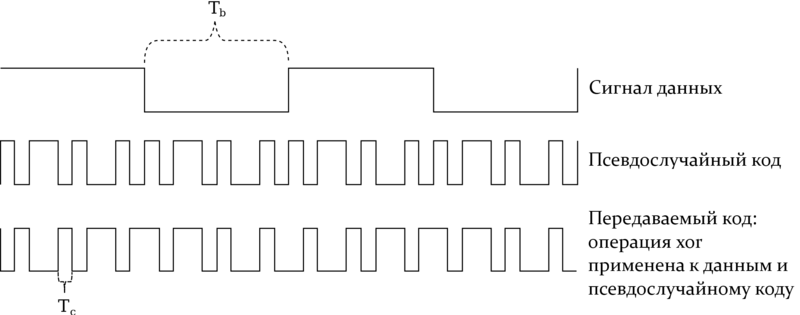
\includegraphics[width=\textwidth]{pic/cdma.png}
\end{center}
DSSS - Direct Sequence Spread Spectrum -- генерация шумоподобного сигнала, занимающего все время и всю полосу (в отличие от FDMA, TDMA)
\end{frame}
%--------------------------------------------------------------------------------
\begin{frame}
\frametitle{CDMA -- множественный доступ с кодовым разделением}
\begin{itemize}
 \item Элементарные последовательности, или чипы:
$$0=\{-1, -1, -1, +1, +1, -1, +1, +1\}$$
$$1=\{+1, +1, +1, -1, -1, +1, -1, -1\}$$
 \item Уменьшение длительности символа $\Rightarrow$ расширение спектра
 \item Каждая станция имеет свою уникальную ортогональную последовательность
 \item Все уникальные последовательности ортогональны между собой
\end{itemize}
\begin{block}{Функции Уолша}
 \begin{itemize}
  \item Система ортогональных функций на пространстве $\{1, -1\}$
  \item Формирование функций -- с помощью строк матриц Адамара
 \end{itemize}

\end{block}

\end{frame}
\begin{frame}
\frametitle{Матрицы Адамара}
\centering
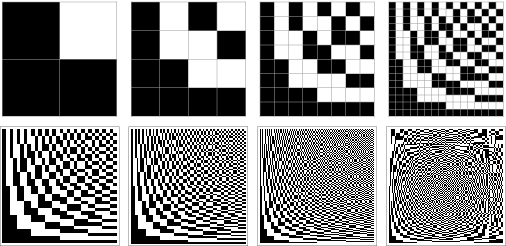
\includegraphics[width=\textwidth]{pic/HadamardMatrices.png}
\end{frame}
%--------------------------------------------------------------------------------
\begin{frame}
\frametitle{Асинхронный CDMA}
\begin{itemize}
 \item Длинные псевдослучайные последовательности практически ортогональны
 \item Низкая взаимная корреляция друг с другом
 \item Автокорреляция мала за исключением нулевого смещения, возможен приём от несинхронизованных станций
 \item Необходимость контролировать мощность передачи, чтобы не нарушить условия взаимной корреляции
\end{itemize}

\end{frame}

%--------------------------------------------------------------------------------
%--------------------------------------------------------------------------------
%--------------------------------------------------------------------------------
\end {document}
